\section{Introduction}

Many techniques exist to determine the position of a user or a device relative to its environment. One possible example is visual positioning, which doesn’t rely on communication-based techniques such as satellite navigation or ultra-wideband (UWB) localization. Visual positioning prevents the necessity of a direct line of sight for signal transmissions or the scattering of beacons inside the building, but it does require that the environment contains enough distinctive landmarks unique to its location. Live camera images are compared to a database of previously recorded images that include positional annotations of said landmarks. If the live image matches one of the database images with high certainty, the user is known to be at the location associated with this database image.

 In this paper, we propose a visual positioning solution for indoor localization at the Museum voor Schone Kunsten (MSK) in Ghent (floor plan shown in figure \ref{fig:msk-groundplan}). This proposal helps visitors by providing the current room number, but more importantly the museum curators themselves. It can give insights on frequently used routes in the museum and show which rooms are more popular based on the number of visitors and the average amount of time spent in that room. Each room contains a large number of recognizable landmarks, the paintings themselves (see figure \ref{fig:image-example}). 

Multiple videos of visitors walking around the museum are available. Besides that, we have access to a dataset that contains the paintings belonging to each room and a testing dataset that contains images with positional annotations of the paintings. Section \ref{sec:preprocessing} presents two image preprocessing steps to improve the overall accuracy and performance of the algorithm. The first technique is a way to sample frames based on how blurry the content is. It prevents the frames from entering other stages of the localization pipeline if needed. This section ends with the calibration procedure of the GoPro camera that was used to record parts of the dataset. The unsupervised painting detector is discussed in section \ref{sec:painting-detection} and includes benchmark performance and common causes of failure. Section \ref{sec:painting-matching} explains the matching procedure against the database. All previous components come together in section \ref{sec:localisation}. By combining all parts and extending it with a hidden Markov model, it is possible to accurately determine the location and return the path taken to its current location.

\begin{figure}[htbp]
    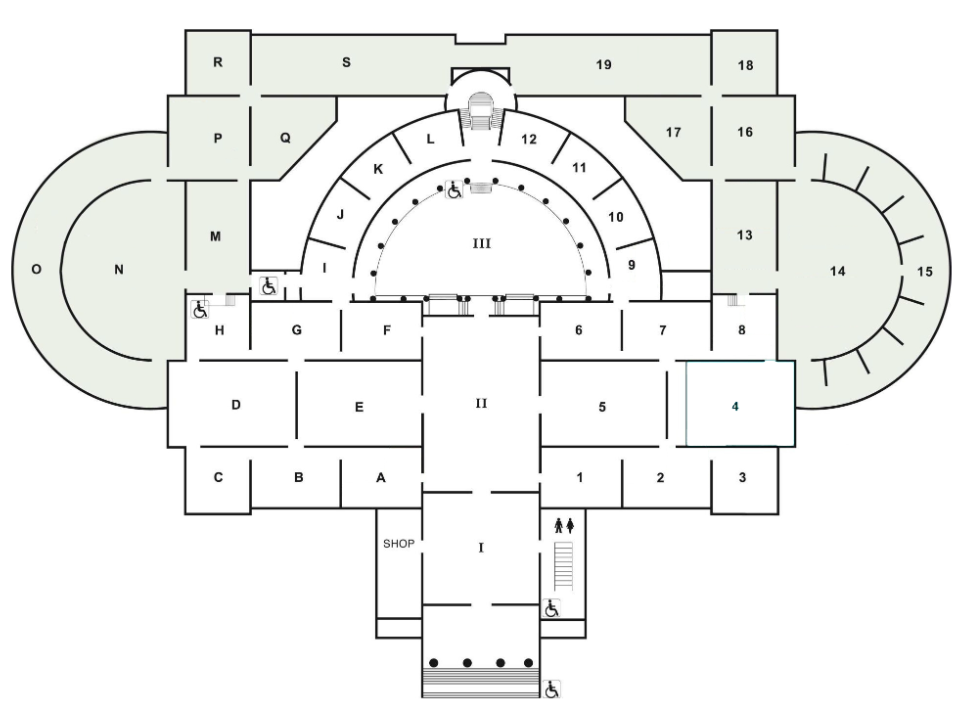
\includegraphics[width=\linewidth]{images/groundplan_msk.PNG}
    \caption{Floor plan of Museum van Schone Kunsten Gent}
    \label{fig:msk-groundplan}
\end{figure}

\begin{figure}[htbp]
    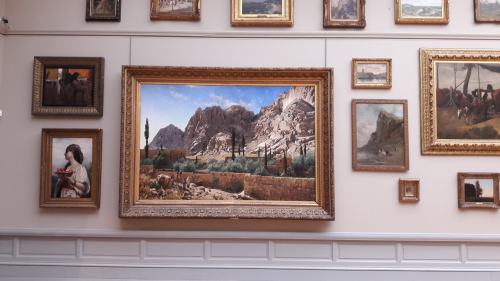
\includegraphics[width=\linewidth]{images/image-example.png}
    \caption{Sample image of the museum}
    \label{fig:image-example}
\end{figure}